

\section{Un premier pas vers la mémoire : les variables}
\begin{UPSTIinfor}{Qu'est-ce qu'une variable ?}
\vspace{1em}
\textbf{Une variable est un espace de stockage pour des données qui peuvent changer au cours de l'exécution du programme.} 

Par exemple, vous pouvez utiliser une variable pour stocker le score d'un jeu ou le nom d'un utilisateur.
\end{UPSTIinfor}

\begin{UPSTIidee}{Analogie}
    On peut imaginer une variable comme une boîte dans laquelle on place des informations. On peut ouvrir cette boîte pour voir ce qu'il y a à l'intérieur, ou y mettre de nouvelles informations.
\end{UPSTIidee}

Sur scratch, on affecte une valeur à une variable en utilisant le bloc "mettre [nom de la variable] à [valeur]".

\subsection{Notre première variable}
\begin{UPSTIManipulation}{Comment créer une variable Scratch ?}
    \begin{itemize}[label=$\square$]
        \item Dans la palette de blocs, trouvez la catégorie "Variables".
        \item Cliquez sur "Créer une variable" et nommez-la comme vous le souhaitez.   
    \end{itemize}
    Un bloc orange arrondi \raisebox{-.3\height}{
\includegraphics[height=2em]{my-variable@4x.png}} apparaît alors dans la palette de blocs, c'est votre variable.
\end{UPSTIManipulation}

\begin{UPSTIManipulation}{Personnaliser le message}
    Notre premier programme était très impersonnel ! Accueillons l'utilisateur avec un message personnalisé. 
    \begin{itemize}[label=$\square$]
        \item Créez une variable appelée "Nom".
        \item Ajoutez un bloc "demander [Quel est votre nom ?] et attendre" avant le bloc "dire".
        \item Le bloc Demander est associé à une variable spéciale appelée "réponse". Ces deux blocs se trouvent dans la catégorie Capteur ("Sensing").
        \item Utilisez le bloc "mettre [Nom] à [réponse]" pour stocker la réponse de l'utilisateur dans la variable "Nom".
        \item Utiliser un bloc "regrouper" pour rassembler "Bonjour" et la variable "Nom" dans le bloc "dire".
        \item Cliquez sur le drapeau vert pour exécuter votre programme. 
        \item Vous devriez voir le sprite demander votre nom et afficher un message personnalisé.
    \end{itemize}
    \begin{minipage}{.5\textwidth}
        \begin{center}
            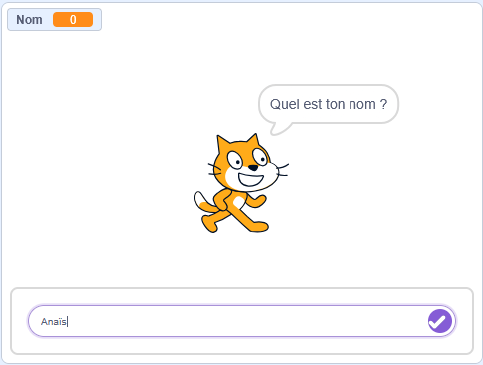
\includegraphics[width=\linewidth]{quel-est-ton-nom.png}
        \end{center}
    \end{minipage}\hfill
    \begin{minipage}{.5\textwidth}
        \begin{center}
            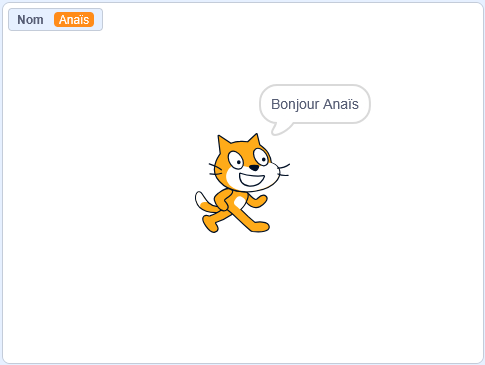
\includegraphics[width=\linewidth]{bonjour_anais.png}
        \end{center}
    \end{minipage}
\end{UPSTIManipulation}

\subsection{Nos premiers calculs}
Notre première variable était un texte, mais on peut aussi utiliser des nombres.
\begin{UPSTIManipulation}{Calculer l'année de naissance}
    \begin{itemize}[label=$\square$]
        \item Créez une variable appelée "Âge" ainsi qu'une variable "Année de naissance".
        \item Ajoutez un bloc "demander [Quel est votre âge ?] et attendre" avant le bloc "dire".
        \item Utilisez le bloc "mettre [Âge] à [réponse]" pour stocker la réponse de l'utilisateur dans la variable "Âge".
        \item Utilisez un bloc "mettre [Année de naissance] à [2025 - Âge]" pour calculer l'année de naissance de l'utilisateur.
        \item Utilisez un bloc "dire" pour afficher "Vous êtes né en [Année de naissance]".
        \item Cliquez sur le drapeau vert pour exécuter votre programme. Vous devriez voir le sprite demander votre âge et afficher l'année de naissance calculée.
    \end{itemize}
\end{UPSTIManipulation}

\subsection{A vous de jouer}

\begin{UPSTIManipulation}{Sprite tient un tacos}
    \begin{itemize}[label=$\square$]
    \item Créer un programme qui demande à l'utilisateur combien de tacos et de kebab il veut commander. 
    \item Ce programmme répondra le montant total de la commande.
    \item Faire valider votre programme par l'enseignant.
    \end{itemize}
\end{UPSTIManipulation}